The evaluation is one of the final phases of this project. In this chapter, we will evaluate different aspects of the projects. 
Here it will be discussed why and how the outcome ended up being what it is today.
This includes how the team worked together, why it gave the result it did, the cooperation with the customer, and how it was working with an overseeing force. Furthermore,we will discuss the issues met during the project, and how the process we used worked for us.
We have chosen to split the evaluation into three major parts, group evaluation, project evaluation and technology evaluation. 
 
 
This is the final phase of this project, the evaluation. Here it will be discussed why and how the outcome
ended up being what it is today.  
The technology evaluation will be a fairly straightforward discussion and evaluation of our experiences with the technology we used in this project.
%_______________________________________________________________________________
\section{Group evaluation}
The group evaluation will discuss the social aspects of the project. 
We will discuss the team dynamics, our goals, how we used our role assignment, risk assessment, the advisor the customer, and other issues regarding group evaluation in general.
The project evaluation will be a discussion of the work process and technical problems we encountered.

\subsection{Team dynamics}

\subsection{Communication}
The communication was done through frequent physical meetings, and if someone had other obligations and they were not able to be precent, then we kept in contact though Facebook. This was a suitable solution for us since the team members were available online nearly all the time. 
This made coordination an easier task, since other members could be consulted at any time. 
Furthermore, our small group size allowed us to get well known with each other, and this made the communication better.

Key words for further writing

working hours and people not showing up in time cuz they did something late at night and then figures it was okay not to show up, then the rest of the group did not show up either.


+pysical meetings
+facebook
+stand ups, could have done more of those
+meetings, did not have weekently, but we asked for them if we neededto

-Not alwas CC in emails to the whole group
-Some members did not get the information when needed 


write something about conflicts resolution?

All in all there wherent personal issues, friends, just discussions regaring solutions to the project. 

\subsection{Goals} 


\subsection{Challanges}

In this section we will elaborate on some of the challenges that we encounter during the project. Some if the issues were minor, and some where lager. The team will in this section reflect on the challanges we had, and why they occured, and what we could have done differently.

\subsubsection{Time}

Throughout the project, time restrictions has been a challange because most of the members in the group have had other projects during the semester. Everyone also had different courses, so suitable working hours for everyone was also a challange. Agnethe had two different projects in addition to the customer driven project. Milos also had another project that was quite time consuming in the beginning. Jan and Tomas also had another project besides the customer driven project, and Jan also wanted to take Norwegian classes. All of this made it hard to find working hours. 

\subsubsection{Language Barriers}


\subsection{Work distribution}

The work distribution was very dynamic. We agreed on what needed to be done, and then group members had to take individual responsibility to perform work on the tasks they were comfortable with.
We could have distributed the work more evenly through out the project. 
It was a little stessful towars the ending of the project. Especially since we had to prioritize making the demo-video in the 5th sprint. Then we had a little trouble with the demo-video, and we had to spend more hours than we first thought. Because of this writing the documentation was a lower priority, and we fell a little behind.  
  
\subsection{motivation}
Motivation turned out to be a major stumbling block in our project. For the
most past, this lack of motivation stems from the complexity of the existing
system we were working on, and the fact that the system was not very well
documented. Throughout the implementation phase, we very often had to ask
our customer for help. This made it ever so slightly demotivating to take on
new tasks, as it meant that our customer told us step by step what you were
12.2. GROUP EVALUATION 137
going to do, where in the system it was going to be done, and how it had to be
implemented. Thus the feeling of independence rarely occurred.
\subsubsection{Effort and estimation}
Throughout the project, time restrictions has been an issue for the group. Most of the 
members in the group have had other group projects during the semester, making it hard to 


\subsection{Role assignment}
As mentioned earlier the role assignment was adapted a bit, so it could fit our project better. Also the roles that was assigned to each group member was more of a guideline, rather than a binding responsibility. This was mainly because or some of the team members this was their first scrum project, and some of the roles requireed more experience and knowlede than the respective goup member had. To solve this problem we often devided the roles over several group members depending on the context and situation. Working with the architechture for example often requireed more than one person responsible. 

When we look back at the role assignment we realize that since we were working with many technologies all of us were unfamiliar in the beginning, it might have been a good idea to make each of the role's responsibility more clear, and maybe spend some time enforcing these responsibilities in the early stages of the project. Also, we should have spent more time finding researching which roles we needed, because some of the roles we assigned we did not use. Even though we decided to embrace this as an equal development team, the roles might have been useful for us. 

These are the roles we assigned, and this is how we evaluated them.

\paragraph{Project Leader}
The project leader was supposed to be responsible for the project progress, and delegate tasks to the other team members. This did not work, because the tasks was prioritized by the customer. If one task was done, the team member had picked the task with the highest priority. All of the team members took responsibility for the progress of the project, and tried to make sure that is went according to the plan. The description also claimed that the Project Leader had final call in arguments, but no group member felt the need to have one person in charge. We chose to embrace this as an equal development team, and that worked well for us.

\paragraph{System Architect}
The system architech was responsible for checiking and analyzing all the layers in the produckt, but this was also something not only one person took responsibility for. 

\paragraph{Scrum Master}
Also the Scrum Master role was assigned to one person originally, but every team member took responsibility for following up on this. It became natural for all of the team members to suggest to have stand ups when we had working hours. It was not always easy too keep track of what the other team members where working on, and this problem occured since the team were not able to have working hours everyday. The reason for this was that the team members had other courses with projects as well, and therefore we were not able to meet up every day. Having the whole team responsible for scrum methodology worked well for us.

\paragraph{Communication Responsible}
This role is the only that was used throughout the whole project was the customer and supervisor contact responsible. Although this was not a high workload, it was easier for both the customer and supervisor to have one person to communicate with when they had questions.  

\paragraph{QA Responsible}
The QA was responsible for the quality of all documents and also the end product, but the whole team felt responsible for delivering a product with good quality. The QA is also supposed to help with determening is stories and acceptance criteria are well defined, and if they satisfy the requirements.The problem we had with this was that it is hard to conduct if the team member responsible is not that experienced with the scrum methodology. A QA is also responsible for organizing testing, and this includes that unit tests are well written, provide developers with high level test cases for the stories, and performing explorotory tesing on early builds, but in our project we did not focus on the testing part. 

\paragraph{Documentation Responsible}
Also this was a role that every team emmber took responsibility for. It was good to have one person resonsible to set up a good structure in the beginning, but when we started writing more of the conents everyone participated where they could. 

\subsection{Risk evaluation}
\subsection{Customer} 
\subsection{Advisor}
%_______________________________________________________________________________
\section{Project Evaluation}
This section will start with an evaluation of the planning phase and our preliminary studies.  
Then we will look at our use of the scrum method, and how we had to modify it for our project, before moving on to a discussion of our conduction of meetings. 
\subsection{Planning}
\subsection{Preliminary Studies}
\subsection{Scrum}
\subsection{Meetings-Summary}
\subsection{Course feedback}
\subsection{Testing}
\subsection{Time usage}
%_______________________________________________________________________________
\section{Technologies and tools evaluation}
In this section you can read about main used technologies and tools during developing.
Emphasis is placed on problems encountered during using these tools and technologies.

\subsection{Android}

\subsection{OpenCV}
OpenCV is an open source computer vision library briefly described in section \ref{subsec:image_processing_library}.
It is a very useful library, which saved the team a lot of time instead of implementing image processing parts themselves
 -- whole light detection module was just enhanced demonstration example of OpenCV functionality.

On the other hand, some problems with this library occurred.
OpenCV Java API is a relatively new and therefore some implementation is missing.
One example of this was described in section \ref{sec:sprint3_implementation}.
This raised a lot of problems, which resulted into discarding of user story.

OpenCV Java API can be therefore counted as a immature product but with a high potential in future, provided OpenCV developers will focus more on this API.
At this moment, new relase 2.4.7 if OpenCV is 44 days late according to the plan\footnote{\url{http://code.opencv.org/projects/opencv/roadmap}} with still 32 opened bugs or new features.

\subsection{Git}
The team adopted Git as its version control system since early phase as described in section \ref{subsec:git}.
Most of the members had experience with some other VCS such as Subversion and therefore the idea of versioning was not new.
On the other hand, three of four members of the team had no experience with Git itself.

Even though Git is a powerful tool with a lot of features, the main reason of using was to share code.
Since development was rather linear, branching was used rarely.
On the other hand, support of releases was used quite often \footnote{\url{https://github.com/dohnto/DigitalLighter/releases}}.
This was very comfortable for creating a final report, when the team could easily see exactly what features were included in each prototype and also it was possible to se the GUI of product in particular phase.

Of course, troubles during merging occurred.
Since merging conflicts can be sometimes demanding and usually requires a lot of knowledge about merging code, sometimes it was impossible for one person to solve it.
These conflicts were in most cases solved by discussion with all interested members.

After all the experience with Git is rather positive. 
It is always good to be able to work with tools, that a lot of companies use in real development.


\subsection{Target Process}
Target Process is a collaborative project management tool described in section \ref{subsec:targetProcessToolDescription}.
This tool was chosen after two another tools were tried.
It is very complex tool for large teams and it provides many different views on project (called boards) and also offers to personalize these views.

This tool was used mainly for a collaboration with customer. 
Before sprint planning, user stories for next sprint were prepared and inserted into Target Process.
Customer could easily prioritize these stories by dragging and dropping.
He could also see spend hours on particular story and also the progress bar depicting progress of this story.

Sometimes, due to lack of a discipline, the spend hours and finished stories and tasks were not filled in time and therefore the retrospective cannot be that precise.
Anyway, Target Process was very mature and useful tool for customer communication with much more features that was for this project necessary.


\subsection{TestFlight}
TestFlight service, described in section \ref{subsec:testflight}, was adopted because of customer proposal.
The service was used in early phases of development for customer comfort when testing the product.

Since the beginning of implementation, some non-reproducible errors occurred in client application.
After some testing, the team suspected TestFlight of those problems.
TestFlight for Android is relatively new service \footnote{\url{http://blog.testflightapp.com/post/49971420302/android}} and there it was decided to discard it from the implementation.
After some time, the team has discovered, that the issues were caused by Android system itself 
%___________-_______________________________________
(REF NEEDED)
%__________________________________________________-
, but the TestFlight was never used again, because the demonstration for customer were performed in form of videos.
 
Therefore it is difficult to evaluate tool, that has been used only for a short period of time.

\subsection{Technical issues}
During testing light detection module, problem situation\footnote{Tested with Samsumg Galaxy S3 and Samsung Galaxy S2.} with mobile devices camera was encountered.
In dark, if a tracked object (mobile phone lighting with single color) or camera itself is moving, everything is working as expected.
But if both object and camera are static, after some time, the camera starts to adjust the colors.
You can see that situation in Figure \ref{fig:screen_colors_in_enviroments}.
This is probably caused by exposure settings, and further research concerning that topic would have to be done.
\begin{figure}[h]
        \centering
        \begin{subfigure}[b]{0.4\textwidth}
                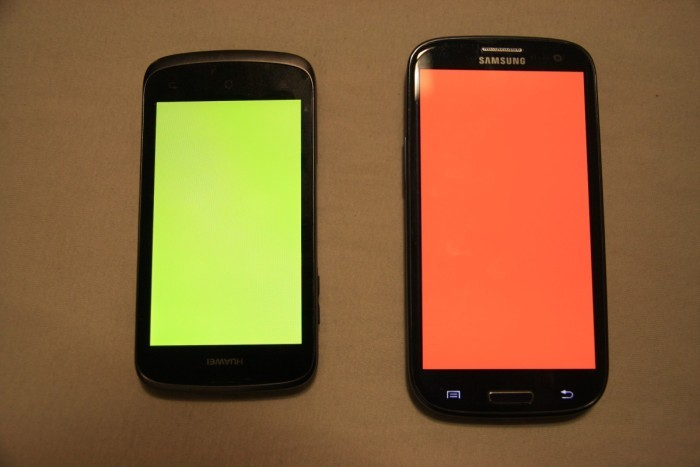
\includegraphics[width=\textwidth]{evaluation/IMG_7029.JPG}
                \caption{Colors of screens in light environment}
                \label{fig:tiger}
        \end{subfigure}
        ~ %add desired spacing between images, e. g. ~, \quad, \qquad etc.
          %(or a blank line to force the subfigure onto a new line)
        \begin{subfigure}[b]{0.4\textwidth}
                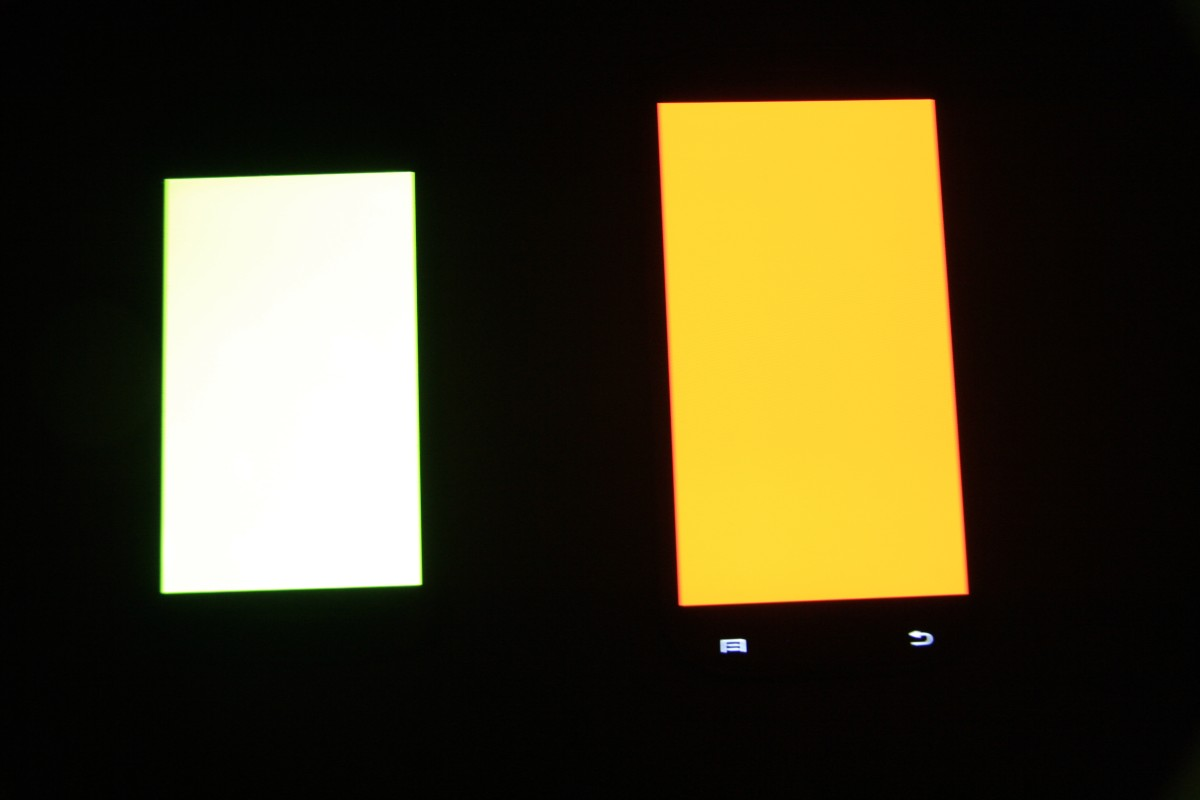
\includegraphics[width=\textwidth]{evaluation/IMG_7032.JPG}
                \caption{Colors of screens in dark environment}
                \label{fig:mouse}
        \end{subfigure}
        \caption{Colors of screens in different light environments}\label{fig:screen_colors_in_enviroments}
\end{figure}
By empirical research there were established colors (e. g. blue and white) which are least affected by this behavior.